\newcommand{\svcourse}{CST Part IA: Software Engineering and Security}
\newcommand{\svnumber}{1}
\newcommand{\svvenue}{Microsoft Teams}
\newcommand{\svdate}{2022-05-11}
\newcommand{\svtime}{15:00}
\newcommand{\svuploadkey}{CBd13xmL7PC1zqhNIoLdTiYUBnxZhzRAtJxv/ytRdM1r7qIfwMsxeVwM/pPcIo8l}

\newcommand{\svrname}{Dr Sam Ainsworth}
\newcommand{\jkfside}{oneside}
\newcommand{\jkfhanded}{yes}

\newcommand{\studentname}{Harry Langford}
\newcommand{\studentemail}{hjel2@cam.ac.uk}


\documentclass[10pt,\jkfside,a4paper]{article}

% DO NOT add \usepackage commands here.  Place any custom commands
% into your SV work files.  Anything in the template directory is
% likely to be overwritten!

\usepackage{fancyhdr}

\usepackage{lastpage}       % ``n of m'' page numbering
\usepackage{lscape}         % Makes landscape easier

\usepackage{verbatim}       % Verbatim blocks
\usepackage{listings}       % Source code listings
\usepackage{graphicx}
\usepackage{float}
\usepackage{epsfig}         % Embed encapsulated postscript
\usepackage{array}          % Array environment
\usepackage{qrcode}         % QR codes
\usepackage{enumitem}       % Required by Tom Johnson's exam question header

\usepackage{hhline}         % Horizontal lines in tables
\usepackage{siunitx}        % Correct spacing of units
\usepackage{amsmath}        % American Mathematical Society
\usepackage{amssymb}        % Maths symbols
\usepackage{amsthm}         % Theorems

\usepackage{ifthen}         % Conditional processing in tex

\usepackage[top=3cm,
            bottom=3cm,
            inner=2cm,
            outer=5cm]{geometry}

% PDF metadata + URL formatting
\usepackage[
            pdfauthor={\studentname},
            pdftitle={\svcourse, SV \svnumber},
            pdfsubject={},
            pdfkeywords={9d2547b00aba40b58fa0378774f72ee6},
            pdfproducer={},
            pdfcreator={},
            hidelinks]{hyperref}

\renewcommand{\headrulewidth}{0.4pt}
\renewcommand{\footrulewidth}{0.4pt}
\fancyheadoffset[LO,LE,RO,RE]{0pt}
\fancyfootoffset[LO,LE,RO,RE]{0pt}
\pagestyle{fancy}
\fancyhead{}
\fancyhead[LO,RE]{{\bfseries \studentname}\\\studentemail}
\fancyhead[RO,LE]{{\bfseries \svcourse, SV~\svnumber}\\\svdate\ \svtime, \svvenue}
\fancyfoot{}
\fancyfoot[LO,RE]{For: \svrname}
\fancyfoot[RO,LE]{\today\hspace{1cm}\thepage\ / \pageref{LastPage}}
\fancyfoot[C]{\qrcode[height=0.8cm]{\svuploadkey}}
\setlength{\headheight}{22.55pt}


\ifthenelse{\equal{\jkfside}{oneside}}{

 \ifthenelse{\equal{\jkfhanded}{left}}{
  % 1. Left-handed marker, one-sided printing or e-marking, use oneside and...
  \evensidemargin=\oddsidemargin
  \oddsidemargin=73pt
  \setlength{\marginparwidth}{111pt}
  \setlength{\marginparsep}{-\marginparsep}
  \addtolength{\marginparsep}{-\textwidth}
  \addtolength{\marginparsep}{-\marginparwidth}
 }{
  % 2. Right-handed marker, one-sided printing or e-marking, use oneside.
  \setlength{\marginparwidth}{111pt}
 }

}{
 % 3. Alternating margins, two-sided printing, use twoside.
}


\setlength{\parindent}{0em}
\addtolength{\parskip}{1ex}

% Exam question headings, labels and sensible layout (courtesy of Tom Johnson)
\setlist{parsep=\parskip, listparindent=\parindent}
\newcommand{\examhead}[3]{\section{#1 Paper #2 Question #3}}
\newenvironment{examquestion}[3]{
\examhead{#1}{#2}{#3}\setlist[enumerate, 1]{label=(\alph*)}\setlist[enumerate, 2]{label=(\roman*)}
\marginpar{\href{https://www.cl.cam.ac.uk/teaching/exams/pastpapers/y#1p#2q#3.pdf}{\qrcode{https://www.cl.cam.ac.uk/teaching/exams/pastpapers/y#1p#2q#3.pdf}}}
\marginpar{\footnotesize \href{https://www.cl.cam.ac.uk/teaching/exams/pastpapers/y#1p#2q#3.pdf}{https://www.cl.cam.ac.uk/\\teaching/exams/pastpapers/\\y#1p#2q#3.pdf}}
}{}


\begin{document}

\begin{enumerate}

    \setcounter{enumi}{1}

    \item Suppose that female pandas who live beyond the age of 20 outnumber male pandas in the same age group by tree to one. How much information, in bits, is gained by learning that a panda that lives 20 is
    male?

    \[
        h(x) = \lg\frac{1}{p(x)} = \lg \frac{1}{\frac{1}{4}} = \lg 4 = 2
    \]

    \item What is the maximum possible entropy $H$ of an alphabet consisting of $N$ different letters? In such a maximum entropy alphabet, what is the probability of its most likely letter? What is the
    probability of its least likely letter?

    Maximum entropy of an alphabet $\Sigma$ occurs when symbols are equiprobable. So the probability of any symbol (namely both the most and least likely symbols) is $\frac{1}{|\Sigma|} = \frac{1}{N}$.

    \item If discrete symbols from an alphabet $S$ having entropy $H(S)$ are encoded into blocks of length $n$ symbols, we derive a new alphabet of symbol blocks $S^n$. If the occurrence of symbols is
    independent, derive the entropy $H(S^n)$ of this new alphabet of symbol blocks.

    The entropy is $H(S^n) = n\cdot H(S)$. I prove this result by induction.

    Case $n = 0$:

    Trivial: we see that in any sequence of \textit{no} symbols there is one result with $p = 1$ (namely the empty sequence) and therefore the entropy is $1 \cdot \lg 1 = 0 = 0 \cdot H(S)$.

    Case $n = k + 1$:

    With the induction hypothesis that $H(S^k) = k \cdot H(S)$.
    \begin{align*}
        H(S^{k + 1})
        &= \sum_{\sigma^{k + 1} \in S^{k + 1}} p(\sigma^{k + 1}) \cdot \lg \frac{1}{p(\sigma^{k + 1})} && \text{\hspace{-12em}Definition of entropy}\\
        &= \sum_{\sigma \in S}\sum_{\sigma^k \in S^k} p(\sigma\sigma^k) \cdot \lg \frac{1}{p(\sigma\sigma^k)} && \text{\hspace{-12em}Definition of $S^{k + 1}$}\\
        &= \sum_{\sigma \in S}\sum_{\sigma^k \in S^k} p(\sigma) \cdot p(\sigma^k) \cdot \lg \frac{1}{p(\sigma) \cdot p(\sigma^k)} && \text{\hspace{-12em}Independence}\\
        &= \sum_{\sigma \in S}\sum_{\sigma^k \in S^k} p(\sigma) \cdot p(\sigma^k) \cdot \lg\frac{1}{p(\sigma)} + p(\sigma) \cdot p(\sigma^k) \cdot \lg \frac{1}{\cdot p(\sigma^k)}\\
        &= \left(\sum_{\sigma \in S} p(\sigma) \cdot \lg\frac{1}{p(\sigma)} \left(\sum_{\sigma^k \in S^k} p(\sigma^k)\right)\right) + \left(\sum_{\sigma \in S} p(\sigma)\right) \cdot
        \left(\sum_{\sigma^k \in S^k} p(\sigma^k) \cdot \lg \frac{1}{\cdot p(\sigma^k)} \right) \\
        &= \left(\sum_{\sigma \in S} p(\sigma) \cdot \lg\frac{1}{p(\sigma)} \right) + \left(\sum_{\sigma^k \in S^k} p(\sigma^k) \cdot \lg \frac{1}{\cdot p(\sigma^k)} \right)
        && \text{\hspace{-12em}Probabilities sum to 1} \\
        &= H(S) + H(S^k)
        && \text{\hspace{-12em}Definition of Entropy} \\
        &= (k + 1) \cdot H(S)
        && \text{\hspace{-12em}Induction Hypothesis}
    \end{align*}

    Thus, since we have that the theorem holds for $n = 0$ and if it holds at $n = k$ then it must also hold at $n = k + 1$; we can conclude that it must hold for \textit{all} $n \in \mathbb{N}$. So we have
    proved the result, as required. Therefore $H(S^n) = n \cdot H(S)$

    \item Why are fixed length codes inefficient for alphabets whose letters are not equiprobable? Discuss this in relation to Morse Code?

    In this case, we have symbols which contain very few shannon bits taking being represented with lots of bits. Consider the case of a random variable $X$ ranging over an alphabet $\Sigma$ with $128$ symbols
    but $H(X) = 3$. If we use fixed-length codes, then we have to use $7$ bits to represent each symbol -- where we could use a variable length code and have an average of $3 + \epsilon$ bits!

    The entropy of letters in English (assuming independence) is $\sim 4.1$ bits per letter: if we use a fixed-length code then we require $\lceil\lg 26 \rceil = 5$ bits per letter.

    Morse Code is a code which exploits this difference: $e$ is the most common letter of the alphabet and is represented with $1$ dot: the shortest possible transmission. While $z$, the least common letter is
    represented with $5$ dots. This make Morse Code more efficient than a fixed-length code.

    \item A fair coin is secretly flipped until the first head occurs. Let $X$ denote the number of flips required. The flipper will truthfully answer any ``yes-no'' questions about his experiment, and we wish
    to discover thereby the value of $X$ as efficiently as possible.

    \begin{enumerate}

        \item What is the most efficient possible sequence of such questions?

        Using the entropy-max principle, the most efficient questions to ask are those for which the answers are equiprobable.

        Therefore, the $i^\mathrm{th}$ question should be ``was the first head at $i$'' (starting at $i = 0$). This guarantees that the answer to the $i^{\mathrm{th}}$ question has a 50\% chance of taking either
        answer. Therefore the information gained from each question is maximised.

        \item On average, how many questions should we need to ask?

        $2$ questions.

        The entropy of $X$ is 2 bits and each question gives $1$ bit of information.
        \begin{align}
            \forall x \in \mathbb{N}_{\ge 1}\ldotp P(x) &= 2^{-x} \\
            H(X)
            &= \sum^{\infty}_{x = 1} p(x) \cdot \lg \frac{1}{p(x)} \\
            &= \sum^{\infty}_{x = 1} 2^{-x} \cdot \lg 2^{x} \\
            &= \sum^{\infty}_{x = 1} x \cdot 2^{-x} \\
            &= \frac12 \cdot \sum^{\infty}_{x = 1} x \cdot \frac12^{x - 1} \\
            &= \frac12 \cdot \frac{1}{\left(1 - \frac12\right)^2} \\
            &= 2
        \end{align}
        So the entropy of when the coin first landed heads is 2 bits and therefore, the number of questions we should need to ask on average is 2.

        \item Relate the sequence of questions to the bits in a uniquely decodable prefix code for $X$.

        The most efficient uniquely decodable prefix code for such a language is a code with variable sizes codes; where ``heads on $i^{\text{th}}$ throw is represented by
        $\underbrace{0\ldots0}_{\times {i - 1}}1$. Each question we ask is checking to see whether the code representing that was the $i^{\text{th}}$.

    \end{enumerate}

    \item Is it possible to construct a prefix code in which the codewords have the following lengths: $1$, $2$, $3$, $3$, $4$, $4$.

    Lets apply the Kraft inequality: for any uniquely decodable code over the alphabet $\Sigma$ with codeword lengths $L = \{\ell_1, \ldots \ell_n\}$
    \[
        \sum_{\ell \in L} |\Sigma|^{-\ell} \le 1
    \]

    For the alphabet $\{0, 1\}$, apply this to the codewords we have:
    \[
        \frac12 + \frac14 + \frac18 + \frac18 + \frac1{16} + \frac1{16} = 1 + \frac18 > 1
    \]
    So, we have that any code with codewords of those lengths over $\{0, 1\}$ does not satisfy the Kraft-inequality and therefore cannot be uniquely decodable. All prefix codes are uniquely decodable and
    therefore it cannot be a prefix code

    However, if we consider an alphabet $|\Sigma| > 2$ (it was never stated that we had to consider $\Sigma = \{0, 1\}$)then the inequality is satisfied and there is a uniquely decodable code (and a prefix code)
    with codewords of that length.

    \item Consider three variable-length codes for a four-symbol alphabet $\{A, B, C, D\}$ having probabilities $p(x)$ as shown:
    \begin{table}[H]

        \centering

        \begin{tabular}{c|c|c|c|c}
            $x$ & $p(x)$ & Code 1 & Code 2 & Code 3 \\
            $A$ & 0.25 & 00 & 0 & 01 \\
            $B$ & 0.5 & 1 & 0 & 0 \\
            $C$ & 0.125 & 01 & 110 & 011 \\
            $D$ & 0.125 & 10 & 111 & 111
        \end{tabular}

    \end{table}

    Compare the average codeword length of each code to the entropy of the alphabet, and for each code give all possible decodings of the bit sequence ``1001'' as a complete message. Which codes are uniquely
    decodable; which have the prefix (instantaneous) property; which code is best, and why?
    \[
        H(X) = \sum_{x \in X} p(x) \cdot \lg \frac{1}{p(x)} = 1.75
    \]

    \begin{align}
        \bar{L_1} &= 0.25 \cdot 2 + 0.5 \cdot 1 + 0.125 \cdot 2 + 0.125 \cdot 2 = 1.5 \\
        \bar{L_2} &= 0.25 \cdot 2 + 0.5 \cdot 1 + 0.125 \cdot 3 + 0.125 \cdot 3 = 1.75 \\
        \bar{L_3} &= 0.25 \cdot 2 + 0.5 \cdot 1 + 0.125 \cdot 3 + 0.125 \cdot 3 = 1.75
    \end{align}

    \begin{table}[H]

        \centering

        \begin{tabular}{c|cc}
            Code 1 & $BAB$ & $DC$ \\
            Code 2 & \\
            Code 3 & \\
        \end{tabular}

        \caption{Decodings of the bit sequence ``1001''}

    \end{table}

    Code 2 and Code 3 are uniquely decodable and are compressed down to entropy. Code 2 is a prefix code. So Code 2 is the best code, since it is a prefix code at the entropy limit and none of the others are.

    \item Find a probability distribution $\{p_1, p_2, p_3, p_4\}$ such that there are two optimal codes that assign different lengths $\{\ell_i\}$ to the four symbols.

    $\left\{\frac13, \frac13, \frac16, \frac16\right\}$. Consider the two codes $\{00, 01, 10, 11\}$ and $\{0, 10, 110, 111\}$. They both have a mean length of $2$.

    \item Construct an ensemble where the difference between the entropy and the expected length of the Huffman code is as large as you can make it.

    Consider the ensemble (of length 1) $\{(a, 1 - \delta), (b, \delta)\}$. Using a Huffman code, we get the code $\{(a, 0), (b, 1)\}$.

    The difference between the entropy and the expected length of the Huffman code is given by:
    \begin{align}
        \Delta
        &= ((1 - \delta) \cdot 1 + \delta \cdot 1) - (1 - \delta) \cdot \lg \frac{1}{1 - \delta} - \delta \cdot \lg \frac{1}{\delta} \\
        &= 1 - (1 - \delta) \cdot \lg \frac{1}{1 - \delta} - \delta \cdot \lg \frac{1}{\delta} \\
        \lim_{\delta \to 0} \Delta &= 1
    \end{align}

    By the limits of Huffman Coding, we have that the expected length of a Huffman Code is \textit{strictly less than} one greater than the entropy of the sequence. Thus, our code is the worst possible case.

    \item You are tasked with investigating a funky random number generator, which generates integers $i$ where $1 \le i \le n$. The true distribution $(p_1, p_2, \ldots, p_n)$ is unknown, but the average $\mu$
    is known. In order to perform inference and estimate the posterior distribution using Bayes theorem, we need a prior distribution.

    \begin{enumerate}

        \item Show, using the method of Lagrange multipliers, that for the maximum entropy prior $p_i$ can be written as $C r^i$ for some $C$ and $r$.

        Start by stating the function we wish to optimise and the constraints:
        \begin{align*}
            H(X) &= \sum p_i \cdot \lg \frac{1}{p_i} \\
            0 &= \sum p_i - 1 && \text{probabilities sum to 1} \\
            0 &= \sum p_i \cdot i - \mu && \text{$\mu$ is the mean} \\
            \intertext{Now, we can form the Lagrangian}
            L &= H(X) + \lambda \cdot \left(\sum p_i - 1\right) + \eta \cdot \left(\sum p_i \cdot i - \mu\right) \\
            \frac{\partial L}{\partial p_i} &= -\lg p_i - 1 + \lambda + \eta \cdot i \\
            \intertext{Now, recall that at maximum entropy, the derivative is zero}
            0 &= -\lg p_i - 1 + \lambda + \eta \cdot i \\
            p_i &= 2^{\lambda - 1} \cdot \left( 2^\eta \right)^i && \text{by rearranging}
        \end{align*}
        Thus, we have that the maximum entropy prior $p_i$ can be written as $C r^i$ for some $C$ and $r$.

        \item Use normalisation to find $C$.

        Using the fact that $\sum p_i = 1$ and these constants are shared between all $p_i$:
        \begin{align}
            \sum^n_{i = 1} p_i &= 1 && \text{probabilities sum to 1} \\
            C \cdot \sum^n_{i = 1} r^i &= 1 && \text{shown above} \\
            C \cdot r \cdot \sum^n_{i = 1} r^{i - 1} &= 1 && \text{rearranging} \\
            C \cdot r \cdot \frac{1 - r^n}{1 - r} &= 1 && \text{formula for sum of a geometric sequence} \\
            C &= \frac{1 - r}{r(1 - r^n))} && \text{rearranging}
        \end{align}
        Thus, we have that $C = \frac{1 - r}{r(1 - r^n)}$.

        \item Use the known average of the distribution to obtain the following equation:
        \[
            n r^{n + 1} - (n + 1) r^n + 1 = \mu (r^n - 1)(r - 1)
        \]
        \begin{align}
            \mu &= \sum^n_{i = 1} p_i \cdot i && \text{by definition of mean} \\
            \mu &= C \cdot \sum^n_{i = 1} r^i \cdot i && \text{expression for $p_i$} \\
            \mu &= \frac{1 - r}{r(1 - r^n)} \cdot \sum^n_{i = 1} r^i \cdot i && \text{expression for $C$} \\
            \mu &= \frac{1 - r}{r(1 - r^n)} \cdot r \cdot \sum^n_{i = 1} r^{i - 1} \cdot i \\
            \mu &= \frac{1 - r}{r(1 - r^n)} \cdot r \cdot \frac{\partial}{\partial r}\left(\sum^n_{i = 1} r^i\right) \\
            \mu &= \frac{1 - r}{1 - r^n} \cdot \frac{\partial}{\partial r}\left(r \cdot \sum^{n}_{i = 1} r^{i - 1}\right) \\
            \mu &= \frac{1 - r}{1 - r^n} \cdot \frac{\partial}{\partial r}\left(\frac{r(1 - r^n)}{1 - r}\right) && \text{sum of a geometric sequence} \\
            \mu &= \frac{1 - r}{1 - r^n} \cdot \frac{(1 - (n + 1) \cdot r^n) \cdot (1 - r) + r \cdot (1 - r^n)}{(1 - r)^2} \\
            \mu &= \frac{1 - r - (n + 1) \cdot r^n + (n + 1) \cdot r^{n + 1} + r - r^{n + 1}}{(1 - r^n) \cdot (1 - r)} \\
            \mu &= \frac{n \cdot r^{n + 1} - (n + 1) \cdot r^n + 1}{(1 - r^n) \cdot (1 - r)}
        \end{align}
        Finally, multiply both sides by $(1 - r^n) \cdot (1 - r)$ to get the required result:
        \[
            n \cdot r^{n + 1} - (n + 1) \cdot r^n + 1 = \mu \cdot (1 - r^n) \cdot (1 - r)
        \]

        \item This equation is difficult to solve analytically, so solve it numerically. For $n = 6$, plot the distribution of $p_i$ for $\mu = 3.5$, $\mu = 2$ and $\mu = 5$.

        \begin{figure}[H]

            \centering

            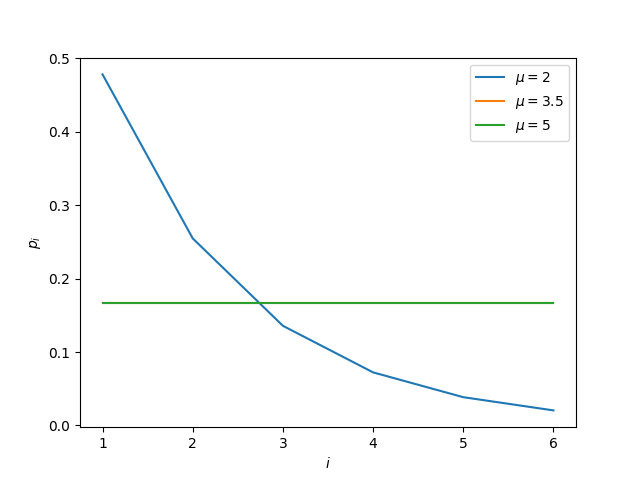
\includegraphics[width=0.5\textwidth]{plot}

            \caption{Prior Distribution according to Principle of Maximum Entropy}

        \end{figure}

        Notice that the distribution for $\mu = 3.5$ and $\mu = 5$ is the same! This is because, for $\mu \ge 3.5$ we have that $r \ge 1$. The equation is \textbf{not valid} for $r \ge 1$ because we had to use
        the sum of a geometric random variable in the derivation: and that equation is only valid for $r < 1$!

    \end{enumerate}

\end{enumerate}

\end{document}
